In this chapter I will describe the high-level architecture of the IoT platform, based on the component diagram.

Internet of Things, as a system, requires outlying units ``on site'', which measure the data and send it to the processing centers.
These units are in my case both the smartwatches and mobile phones.

The smartwatch requires an application to propagate the data from the heart rate sensor to the mobile application through the \code{hr\_data} interface.
Once the raw data is received, it is combined with GPS data from the phone and forwarded through the \code{data\_access} interface to the IoT platform, where it gets processed and saved.
When the smartphone application requires it, it requests the processed data through the same interface and displays it.

\begin{figure}[h]
    \tmpframe{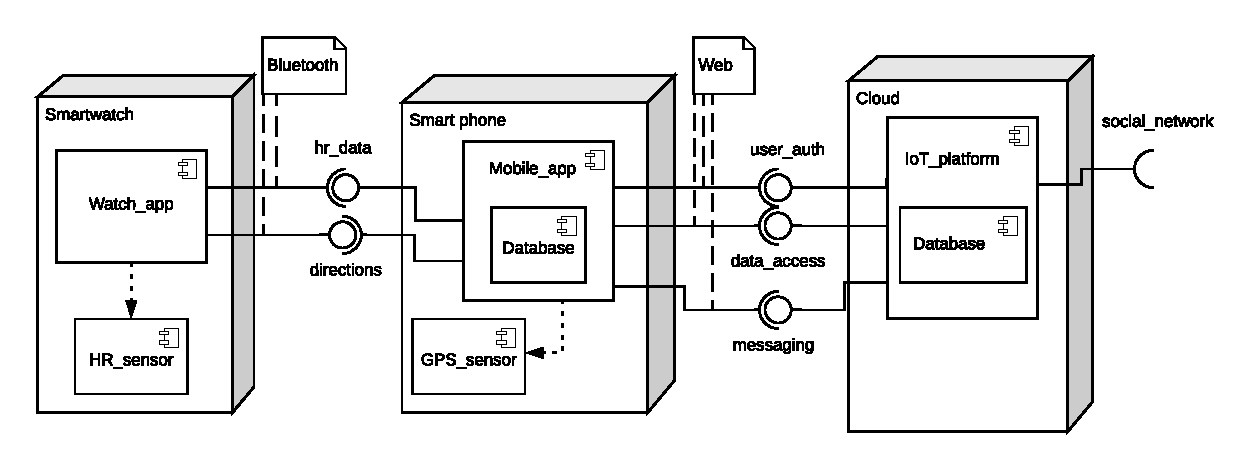
\includegraphics[width=\textwidth]{Images/component.pdf}}
    \caption{Component diagram of the designed IoT solution.}
\end{figure}

Depending on the number and complexity of the features in the future, it is also possible to introduce a web client in order to make the smartphone APP lighter and easier to navigate.

The watch communicates with the phone application over Bluetooth, with the phone application acting as a server, waiting for the watch application to connect and send its data.
The phone application connects to the server using the phone's Internet connection.

\section{Smartwatch application}
Since the vendors of smartwatches generally use proprietary operating systems, every integrated smartwatch type needs an application of its own.
This is distributed together with the phone application.

Generally, it should be as light-weight as possible, to spare the limited battery resources.
Without any need for persistence, the application layer should collect the data from the heart rate sensors and regularly send them to the phone in batches.
The presentation layer displays data from the phone (such as instructions for a fitness test or navigation directions) received through the \code{directions} interface.
This is why it requires a bi-directional channel for Bluetooth communication.

\section{Smartphone application}
The phone application needs to be able to communicate with the watch via Bluetooth using the \code{hr\_data} and \code{directions} interfaces, as well as with the APIs for data access, notification and  user authentication offered by the server.

The user is authenticated via \code{user\_auth}.

The \code{Database} also contains the user's plans, so that the user does not have to be online when in navigation mode.

When navigating, the \code{Mobile\_app} collects data from the available \linebreak\code{GPS\_sensor} and from the \code{Watch\_app}, and tries to send it to the server via the \code{data\_access} interface if there is an active Internet connection.
Otherwise this is stored in the local \code{Database} and sent when the phone next connects.

The \code{Mobile\_app} is also subscribed to a messaging service such as Firebase~\cite{firebase} provided by the server to handle notifications.

\section{Server application}
The \code{IoT\_platform} application communicates with the \code{Mobile\_app} via the aforementioned interfaces, and also requires a public interface from every supported social network, so that the users can log in using their accounts from those networks and add new friends that they already know.

The server application has a simple front-end client for administration purposes.

The \code{IoT\_platform} is hosted in a cloud, since this infrastructure provides room for scalability and performance~\cite{cloud},
which should work perfectly in combination with my application's need for storing of detailed route definitions and computing tailored route difficulty estimates.

The offered \code{user\_auth} interface is used for authentication.
The user's data should be as secure as possible given its very personal nature, while maintaining a comfortable level of usability for the user;
this is why authentication should be done with OAuth, as opposed to HTTP Basic Auth, combined with a One Time Password for logins from unrecognized devices.
